% Asset ID: FAS2ProductMomentCorrelationCoefficientTikZ-002
% Unit: FAS2
% Topic code: FAS2-BIV
% Topic ID: FAS2ProductMomentCorrelationCoefficient
% Related lesson file: FAS2_product_moment_correlation_coefficient_lesson.md
% Used placeholder:
% [VISUAL PLACEHOLDER: FAS2ProductMomentCorrelationCoefficientTikZ-002 | Source: AI-proposed teaching enhancement based on PMCC limitations | Insert from tikz/FAS2ProductMomentCorrelationCoefficientTikZ-002.tex | Purpose: Show why r ≈ 0 does not always mean no pattern. Description: Contrast a random cloud with a clear U-shaped non-linear pattern, both labelled as having little/no linear correlation.]
% Source: AI-proposed teaching enhancement based on transcript limitation that r measures linear correlation only.
% Purpose: Show why r close to 0 means little/no linear correlation, not necessarily no relationship.

\documentclass[tikz,border=8pt]{standalone}
\usepackage{amsmath}
\usepackage{xcolor}
\definecolor{Canvas}{HTML}{FAF9F6}
\definecolor{Ivory}{HTML}{FFFFF0}
\definecolor{Ink}{HTML}{2C2C2E}
\definecolor{LineSoft}{HTML}{E5E5EA}
\definecolor{Gold}{HTML}{C5A059}
\definecolor{Blush}{HTML}{FBEFEF}
\begin{document}
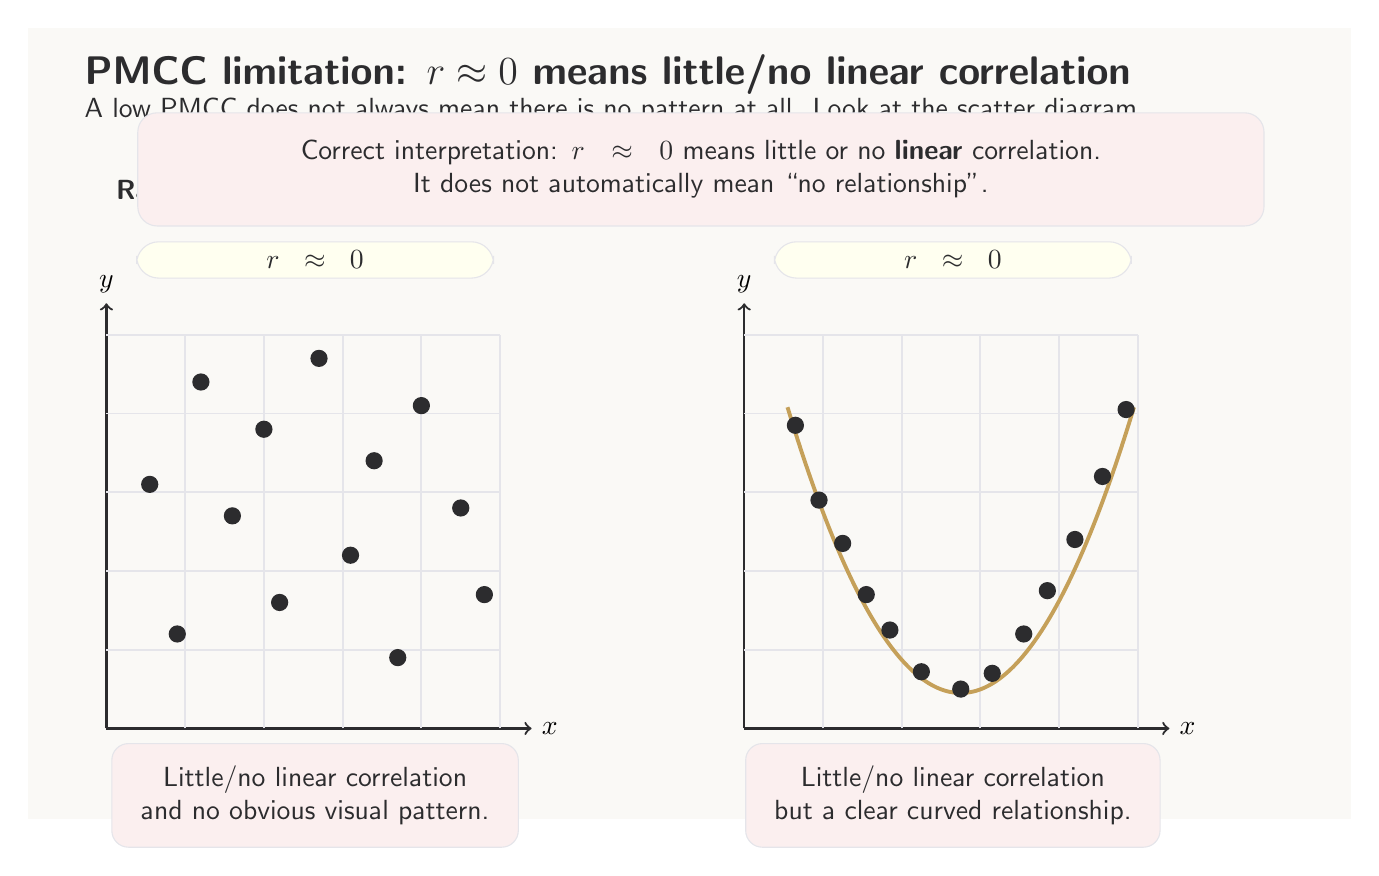
\begin{tikzpicture}[font=\sffamily,axis/.style={->, thick, draw=Ink},guide/.style={draw=LineSoft, line width=0.7pt},data/.style={circle, fill=Ink, inner sep=2.2pt},note/.style={rounded corners=6pt,draw=LineSoft,fill=Blush,text=Ink,align=center,inner sep=8pt}]
\fill[Canvas] (-1,-1.15) rectangle (15.8,8.9);
\node[anchor=west, text=Ink, font=\sffamily\bfseries\Large] at (-0.4,8.3) {PMCC limitation: \(r\approx 0\) means little/no \emph{linear} correlation};
\node[anchor=west, text=Ink, font=\sffamily\normalsize] at (-0.4,7.85) {A low PMCC does not always mean there is no pattern at all. Look at the scatter diagram.};
\begin{scope}[shift={(0,0)}]
\node[anchor=west, text=Ink, font=\sffamily\bfseries] at (0,6.8) {Random-looking cloud};
\draw[axis] (0,0) -- (5.4,0) node[right] {\(x\)}; \draw[axis] (0,0) -- (0,5.4) node[above] {\(y\)};
\foreach \x in {1,2,3,4,5} {\draw[guide] (\x,0) -- (\x,5);} \foreach \y in {1,2,3,4,5} {\draw[guide] (0,\y) -- (5,\y);} 
\foreach \x/\y in {0.55/3.1,0.9/1.2,1.2/4.4,1.6/2.7,2.0/3.8,2.2/1.6,2.7/4.7,3.1/2.2,3.4/3.4,3.7/0.9,4.0/4.1,4.5/2.8,4.8/1.7} {\node[data] at (\x,\y) {};}
\node[note, text width=4.6cm] at (2.65,-0.85) {Little/no linear correlation\\and no obvious visual pattern.};
\node[rounded corners=8pt,draw=LineSoft,fill=Ivory,text=Ink,text width=4.3cm,align=center] at (2.65,5.95) {\(r\approx 0\)};
\end{scope}
\begin{scope}[shift={(8.1,0)}]
\node[anchor=west, text=Ink, font=\sffamily\bfseries] at (0,6.8) {Clear non-linear pattern};
\draw[axis] (0,0) -- (5.4,0) node[right] {\(x\)}; \draw[axis] (0,0) -- (0,5.4) node[above] {\(y\)};
\foreach \x in {1,2,3,4,5} {\draw[guide] (\x,0) -- (\x,5);} \foreach \y in {1,2,3,4,5} {\draw[guide] (0,\y) -- (5,\y);} 
\draw[Gold, line width=1.4pt, domain=0.55:4.95, smooth, samples=80] plot (\x,{0.45 + 0.75*(\x-2.75)^2});
\foreach \x/\y in {0.65/3.85,0.95/2.90,1.25/2.35,1.55/1.70,1.85/1.25,2.25/0.72,2.75/0.50,3.15/0.70,3.55/1.20,3.85/1.75,4.20/2.40,4.55/3.20,4.85/4.05} {\node[data] at (\x,\y) {};}
\node[note, text width=4.7cm] at (2.65,-0.85) {Little/no linear correlation\\but a clear curved relationship.};
\node[rounded corners=8pt,draw=LineSoft,fill=Ivory,text=Ink,text width=4.3cm,align=center] at (2.65,5.95) {\(r\approx 0\)};
\end{scope}
\node[rounded corners=7pt,draw=LineSoft,fill=Blush,text=Ink,align=center,inner sep=10pt,text width=13.6cm] at (7.55,7.1) {Correct interpretation: \(r\approx 0\) means little or no \textbf{linear} correlation.\\ It does not automatically mean ``no relationship''.};
\end{tikzpicture}
\end{document}
